\section{4(1)-tree comparison}\label{7-dipole}



In this section we will prove the first part of Theorem \ref{T=>CTIL:CTIL}.
Note that according to Proposition~\ref{prop:cost-convex=CTIL+MTW}, it is sufficient to show that if a Riemannian manifold $M$ satisfies 4(1)-tree comparison, then it is CTIL and MTW.
These two conditions will be proved separately.

\begin{thm}{Proposition}\label{prop:CTIL}
Any complete cost-convex Riemannian manifold is CTIL.
\end{thm}

\parit{Proof.}
Assume the contrary; that is, there is $p\in M$ and $u,v\zz\in \TIL_p$ such that $w=\tfrac12\cdot(u+v)\notin \TIL_p$.

Let $\tau$ be the maximal value such that the geodesic $\gamma(t)=\exp_p(w\cdot t)$ is a length-minimizing on $[0,\tau]$.
Set $w'=\tau\cdot w$.
Note that $\tau<1$ and $w'\in\partial \TIL_p$.


Set $q=\exp_p w'$.
By general position argument, we can assume that there are at least two minimizing geodesics connecting $p$ to $q$; see \cite{karcher}.
That is, there is $w''\in \partial \TIL_p$ such that $w''\ne w'$ and $\exp_pw'=\exp_pw''$.

\begin{center}
\begin{lpic}[t(-0 mm),b(-0 mm),r(0 mm),l(0 mm)]{pics/7-config(1)}
\lbl[r]{1.5,32;$x$}
\lbl[l]{59.5,31;$y$}
\lbl[t]{18.5,2;$y'$}
\lbl[t]{32.5,2;$x'$}
\lbl[t]{26,4.5;$p$}
\lbl[r]{22.5,16;$z$}
\lbl[r]{25,32;$q$}
\lbl[l]{28.5,27;$q'$}
\end{lpic}
\end{center}

Fix small positive real numbers $\delta,\eps$ and $\zeta$.
Consider the points
\begin{align*}
q'=q'(\eps)&=\exp_p(1-\eps)\cdot w',
&
z=z(\zeta)&=\exp_p(\zeta\cdot w''),
\\
x&=\exp_p u,
&
x'=x'(\delta)&=\exp_p (-\delta\cdot u),
\\
y&=\exp_p v,
&
y'=y'(\delta)&=\exp_p (-\delta\cdot v).
\end{align*}

We will  show that for some choice of $\delta,\eps$ and $\zeta$ the $p/xx'yy'(q'/z)$-tree comparison does not hold.

Assume contrary, that is, given any small positive numbers $\delta,\eps$ and $\zeta$, there is a point array $\~p$, $\~x$, $\~x'(\delta)$, $\~y$, $\~y'(\delta)$, $\~q'(\eps)$, $\~z(\zeta)\in\HH$ as in the definition of $T$-tree comparison;
that is, the distances between the points in this array are at least as big as the distances of corresponding points in $M$ and the equality holds for the pair adjacent in $p/xx'yy'(q'/z)$.


\hide
\begin{wrapfigure}{r}{35 mm}
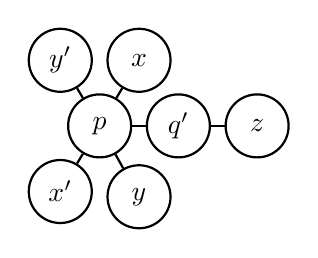
\begin{tikzpicture}[scale=1,
  thick,main node/.style={circle,draw,font=\sffamily\bfseries,minimum size=8mm}]

  \node[main node] (0) at (3/2,11/6){$x$};
   \node[main node] (1) at (1/2,1/6){$x'$};
  \node[main node] (2) at (3/2,.1){$y$};
  \node[main node] (3) at (1,1){$p$};
  \node[main node] (4) at (1/2,11/6){$y'$};
  \node[main node] (5) at (3,1){$z$};
  \node[main node] (6) at (2,1){$q'$};

  \path[every node/.style={font=\sffamily\small}]
     (0) edge node[above]{}(3)
   (1) edge node[above]{}(3)
   (2) edge node[above]{}(3)
   (3) edge node[above]{}(6)
   (4) edge node[above]{}(3)
   (5) edge node[above]{}(6);
\end{tikzpicture}
\end{wrapfigure}
\unhide

Since $\delta$ is small, we can assume that $p$ lies on a necessary unique minimizing geodesic $[x,x']_M$.
Hence 
\[|x-x'|_M=|x-p|_M+|p-x'|_M.\]
By comparison
\begin{align*}
|\~x-\~x'|_\HH&\ge|x-x'|_M,
\\
|\~x-\~p|_\HH&=|x-p|_M,
\\
|\~x'-\~p|_\HH&=|x'-p|_M.
\end{align*}
By triangle inequality,
\[|\~x-\~x'|_\HH=|\~x-\~p|_\HH+|\~x'-\~p|_\HH;\]
that is, $\~p\in [\~x,\~x']_\HH$.
The same way we see that $\~p\in [\~y,\~y']_\HH$.

Fix $\eps$ and $\zeta$.
Note that as $\delta\to 0$ we have 
\begin{align*}
\~x'&\to \~p,
&
\~y'&\to \~p.
\\
\measuredangle[\~p\,^{\~x'}_{\~y}]&\to \measuredangle[p\,^{x'}_{y}],
&
\measuredangle[\~p\,^{\~y'}_{\~x}]&\to \measuredangle[p\,^{y'}_{x}],
\\
\measuredangle[\~p\,^{\~x'}_{\~q'}]&\to \measuredangle[p\,^{x'}_{q'}],
&
\measuredangle[\~p\,^{\~y'}_{\~q'}]&\to \measuredangle[p\,^{y'}_{q'}],
\end{align*}
It follows that 
\begin{align*}
\measuredangle[\~p\,^{\~x}_{\~y}]&\to \measuredangle[p\,^x_y],
&
\measuredangle[\~p\,^{\~x}_{\~q'}]&\to \measuredangle[p\,^x_{q'}],
&
\measuredangle[\~p\,^{\~y}_{\~q'}]&\to \measuredangle[p\,^y_{q'}].
\end{align*}


Therefore, passing to a partial limit as $\delta\to0$, we get a configuration of 5 points 
$\~p, \~x,\~y,\~q'=\~q'(\eps),\~z=\~z(\zeta)$ such that  
\begin{align*}
\measuredangle[\~p\,^{\~x}_{\~y}]&= \measuredangle[p\,^{x}_{y}],
&
\measuredangle[\~p\,^{\~y}_{\~q'}]&= \measuredangle[p\,^{y}_{q'}],
&
\measuredangle[\~p\,^{\~x}_{\~q'}]&= \measuredangle[p\,^{x}_{q'}].
\end{align*}
In other words, the map sending 4 points $0,u,v,w'\in\T_p$ to $\~p,\~x,\~y,\~q\in\HH$ correspondingly is distance preserving.

Note that $q'\to q$ as $\eps\to0$. 
Therefore, in the limit,
we get a configuration $\~p$, $\~x$, $\~y$, $\~q'$, $\~z=\~z(\zeta)$ such that in addition we have
\begin{align*}
|\~q'-\~z|&=|q-z|,
&
|\~p-\~z|&\ge |p-z|,
\\
|\~x-\~z|&\ge |x-p|,
&
|\~y-\~z|&\ge |y-z|
\end{align*}

Since $w''\ne w'$, for small values $\zeta$ the last three inequalities 
imply 
\[|\~q'-\~z|>|q-z|,\]
a contradiction.


\begin{thm}{Proposition}\label{prop:CTIL}
Any cost-convex CTIL Riemannian manifold is MTW.
\end{thm}


\parit{Proof.}
Fix a hinge $[p\,^x_y]$ in $M$; from above $M$ is CTIL.
Therefore $[p\,^x_y]$ has a median; denote it by $[p,q]$.
For $\delta>0$, define $x'=x'(\delta)$ and $y'=y'(\delta)$ as above.

\hide
\begin{wrapfigure}{r}{35 mm}
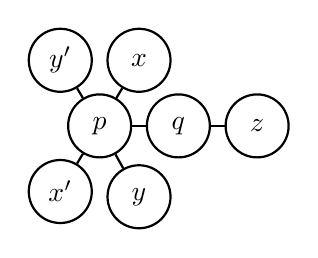
\begin{tikzpicture}[scale=1,
  thick,main node/.style={circle,draw,font=\sffamily\bfseries,minimum size=8mm}]

  \node[main node] (0) at (3/2,11/6){$x$};
   \node[main node] (1) at (1/2,1/6){$x'$};
  \node[main node] (2) at (3/2,.1){$y$};
  \node[main node] (3) at (1,1){$p$};
  \node[main node] (4) at (1/2,11/6){$y'$};
  \node[main node] (5) at (3,1){$z$};
  \node[main node] (6) at (2,1){$q$};

  \path[every node/.style={font=\sffamily\small}]
     (0) edge node[above]{}(3)
   (1) edge node[above]{}(3)
   (2) edge node[above]{}(3)
   (3) edge node[above]{}(6)
   (4) edge node[above]{}(3)
   (5) edge node[above]{}(6);
\end{tikzpicture}
\end{wrapfigure}
\unhide

Without loss of generality we can assume that $x,y\zz\in\exp_p(\TIL_p)$.
If $\delta$ is small, the latter implies that $p$ lies on unique minimizing geodesics $[x,x']$ and $[y,y']$.

Consider the limit case of $p/xx'yy'(q/z)$-comparison  as $\delta\to 0$.
It gives a configuration of 5 points $\~p$, $\~q$, $\~x$, $\~y$ and $\~z$ such that
\begin{align*}
\measuredangle[\~p\,^{\~x}_{\~y}]&=\measuredangle[p\,^x_y],
\end{align*}
$\~q$ is the midpoint of $[\~x, \~y]$.
In particular,
\begin{align*}
2\cdot|\~z-\~q|_\HH^2+|\~q-\~x|_\HH^2+|\~q-\~y|_\HH^2
&=
|\~z-\~x|_\HH^2+|\~z-\~y|_\HH^2,
\\
2\cdot|\~p-\~q|_\HH^2+|\~q-\~x|_\HH^2+|\~q-\~y|_\HH^2
&=
|\~p-\~x|_\HH^2+|\~p-\~y|_\HH^2,
\end{align*}

By the comparison,
\begin{align*}
|\~z-\~x|_\HH&\ge |z-x|_M,
&
|\~z-\~y|_\HH&\ge |z-y|_M,
\\
|\~p-\~x|_\HH&\ge |p-x|_M,
&
|\~p-\~y|_\HH&\ge |p-y|_M,
\\
|\~q-\~x|_\HH&= |q-x|_M,
&
|\~q-\~y|_\HH&= |q-y|_M,
\\
|\~q-\~z|_\HH&= |q-z|_M,
&
|\~q-\~p|_\HH&= |q-p|_M,
\end{align*}
Therefore
\begin{align*}
2\cdot|z-q|_M^2+|q-x|_M^2+|q-y|_M^2
&\ge
|z-x|_M^2+|z-y|_M^2,
\\
2\cdot|p-q|_M^2+|q-x|_M^2+|q-y|_M^2
&\le
|p-x|_M^2+|p-y|_M^2.
\end{align*}
Hence the condition in \ref{MTW} follows.
\qeds


